% ==============================================================================
% Chapter 9: V–A Structure from 5D Chiral Localization
% Status: [Dc] — Derived from 5D Dirac + EDC postulates
% ==============================================================================

\section{V–A Structure from 5D Chiral Localization}
\label{sec:ch9_va_structure}

\begin{tcolorbox}[edcGuardrail, title=\textbf{Epistemic Status}]
This section derives the effective 4D V–A (left-chiral) current structure
from the EDC 5D$\to$4D reduction. The derivation uses:
\begin{itemize}[nosep]
    \item Standard 5D Dirac equation with position-dependent mass \tagBL{}
    \item Domain-wall zero mode localization (Jackiw--Rebbi, Kaplan) \tagBL{}
    \item EDC postulate: Plenum inflow determines mass profile sign \tagP{}
\end{itemize}
The result---that only left-handed modes couple at the interface---is
\textbf{derived} \tagDc{}, not assumed.
\end{tcolorbox}

% ==============================================================================
\subsection{The Physical Picture: What Happens in 5D?}
\label{sec:ch9_physical_picture}

Before writing any equations, let us watch the ``movie'' of what happens in the
fifth dimension. This subsection gives the physical story; the mathematical
derivation follows in subsequent sections.

% --- THE MOVIE ---

\subsubsection{The Setup: A Universe with Depth}

Imagine you are a 4D observer living on a thin membrane---the ``brane''---embedded
in a larger 5D space. You cannot travel into the fifth dimension $z$, but particles
can have profiles that extend into it.

\textbf{What is $z$?} The coordinate $z$ measures distance perpendicular to the
brane. At $z = 0$ sits the observer boundary---the surface where we make measurements.
As $z$ increases, we move ``into the bulk,'' away from observer space.

\textbf{What is the brane?} The brane is a 4D hypersurface where ordinary matter
is localized. Think of it as the floor of a swimming pool: particles are waves
on the surface, but the pool has depth ($z > 0$).

\textbf{What does an observer see?} A 4D observer sees only the ``shadow'' of
5D fields projected onto the boundary. The strength of a particle's interaction
depends on how much of its wavefunction sits at the boundary.

% --- CHIRALITY FILTER ---

\subsubsection{The Chirality Filter: Why Only Left-Handed?}

Here is the key physical insight, stated in one sentence:

\begin{center}
\fbox{\parbox{0.85\textwidth}{\centering
\textbf{The chirality filter:} Left-handed modes are pulled toward the boundary
by the 5D mass gradient; right-handed modes are pushed away into the bulk.
}}
\end{center}

Why does this happen? The mechanism is elegantly simple:

\textbf{Step 1: Energy flows inward.} In EDC, the Plenum (the 5D energy fluid)
flows toward the observer boundary. This is the fundamental asymmetry that
breaks left-right symmetry.

\textbf{Step 2: The inflow creates a mass gradient.} The flowing Plenum exerts
stress on fermion fields. Near the boundary, fermions feel less stress; deeper
in the bulk, they feel more. This creates a position-dependent mass $m(z)$ that
grows with depth.

\textbf{Step 3: The mass gradient acts like a potential.} A left-handed fermion
in this background experiences an effective force \emph{toward} the boundary
(like a ball rolling downhill). A right-handed fermion experiences a force
\emph{away} from the boundary (like trying to push a ball uphill---it rolls away).

\textbf{Step 4: Localization follows.} Left-handed modes pile up at $z = 0$;
right-handed modes spread into the bulk and become dilute.

% --- OVERLAP AND COUPLING ---

\subsubsection{Overlap Determines Coupling}

Now we can understand why left-handed particles interact and right-handed
particles do not.

\textbf{The principle:} Interaction strength equals wavefunction overlap at the
boundary.

Imagine two flashlights shining on a single screen: the overlap of their beams
determines how much they interact. Similarly, if a gauge boson (like the $W$)
lives at the boundary, it can only ``see'' the part of a fermion wavefunction
that also lives there.

\textbf{Left-handed fermions:} Their wavefunction $f_L(z)$ is peaked at $z = 0$.
Most of the probability density sits right at the boundary. The overlap with
a boundary-localized gauge field is order one: full coupling.

\textbf{Right-handed fermions:} Their wavefunction $f_R(z)$ is peaked deep in
the bulk. Only an exponentially small tail reaches the boundary. The overlap
is exponentially suppressed: negligible coupling.

This is the geometric origin of parity violation in weak interactions.

% --- WHAT WE DERIVE VS NOT ---

\subsubsection{What We Derive and What We Do Not}

\begin{tcolorbox}[colback=blue!5, colframe=blue!50!black,
    title=\textbf{Scope of This Chapter}]

\textbf{What this chapter DERIVES} \tagDc{}:
\begin{itemize}[nosep]
    \item Left-handed modes are boundary-localized
    \item Right-handed modes are bulk-displaced
    \item Effective weak coupling is purely V$-$A
    \item Chirality selection follows from inflow direction, not gauge assignments
\end{itemize}

\textbf{What this chapter does NOT derive} (open):
\begin{itemize}[nosep]
    \item The origin of SU(2)$_L$ gauge symmetry---why this particular group?
    \item The W$^\pm$ and Z$^0$ boson masses---Higgs mechanism not addressed
    \item The numerical value of $G_F$---see Chapter 11
    \item CKM/PMNS mixing matrices---generational structure not derived
    \item Neutrino masses and Dirac vs.\ Majorana nature
\end{itemize}

\textbf{Epistemic tags:}
\begin{itemize}[nosep]
    \item Plenum inflow direction: \tagP{} (EDC postulate)
    \item Mass-from-stress coupling: \tagP{} (physical hypothesis)
    \item Domain-wall localization math: \tagBL{} (established physics)
    \item V$-$A emergence from localization: \tagDc{} (derived here)
\end{itemize}
\end{tcolorbox}

% ==============================================================================
\subsection{Purpose and Scope}
\label{sec:ch9_purpose}

With the physical picture in mind, we now state the mathematical problem.

\subsubsection{The Observational Fact}

The weak interaction in 4D couples exclusively to left-handed fermions,
producing the $V{-}A$ current structure:
\begin{equation}
    \mathcal{L}_{\text{weak}} \propto \bar\psi \gamma^\mu (1 - \gamma^5) \psi \, W_\mu
    \label{eq:ch9_va_current}
\end{equation}
This is an observed fact \tagBL{}. The question is: \emph{why}?

\subsubsection{The Standard Model Approach}

In the Standard Model, left-right asymmetry is \emph{imposed} by assigning
different gauge quantum numbers to $\psi_L$ and $\psi_R$. Left-handed fermions
form doublets under SU(2)$_L$; right-handed fermions are singlets. This is
consistent, but it is an \emph{input}, not an explanation.

\subsubsection{The EDC Approach}

In EDC, we seek a \emph{geometric origin}: chirality selection as a consequence
of the 5D structure, not an input. The asymmetry should arise from physics,
not from ad hoc quantum number assignments.

\paragraph{Minimal assumptions.}
We use only:
\begin{enumerate}[nosep]
    \item The 5D Dirac equation with $z$-dependent mass $m(z)$ \tagBL{}
    \item The EDC postulate that Plenum flows toward the observer boundary \tagP{}
    \item The physical coupling of fermion mass to Plenum stress \tagP{}
\end{enumerate}

\paragraph{Scope and limitations.}
\begin{itemize}[nosep]
    \item This chapter addresses chirality selection, not SU(2)$_L$ gauge unification.
    \item CKM/PMNS mixing is not derived here; it remains (open).
    \item The numerical value of $G_F$ is not computed; see Ch.~11 for the pathway.
\end{itemize}

% ==============================================================================
\subsection{5D Dirac Field and Chiral Decomposition}
\label{sec:ch9_dirac}

We now write the equations. Remember: these equations \emph{formalize} the
physical picture from Section~\ref{sec:ch9_physical_picture}, not replace it.

\subsubsection{The 5D Dirac Equation}

\textbf{The setup.} Consider a fermion field $\Psi(x^\mu, z)$ in the 5D EDC geometry.
The coordinates are $x^M = (x^\mu, z)$ where $\mu = 0,1,2,3$ and $z$ is
the fifth dimension (perpendicular to the brane).

\textbf{The equation.} The 5D Dirac equation with position-dependent mass is \tagBL{}:
\begin{equation}
    \left( i\gamma^\mu \partial_\mu + i\gamma^5 \partial_z - m(z) \right) \Psi = 0
    \label{eq:ch9_5d_dirac}
\end{equation}
This is the standard Dirac equation, except that the mass is not a constant---it
depends on where you are in the fifth dimension.

\textbf{What each term does:}
\begin{itemize}[nosep]
    \item $\gamma^\mu$ are the standard 4D Dirac matrices, $\{\gamma^\mu, \gamma^\nu\} = 2\eta^{\mu\nu}$
    \item $\gamma^5 = i\gamma^0\gamma^1\gamma^2\gamma^3$ is the chirality operator
    \item $m(z)$ is the position-dependent fermion mass (to be determined by EDC physics)
\end{itemize}

The key is the term $i\gamma^5 \partial_z$: it couples left-handed and right-handed
components differently to the $z$-direction. This is where chirality enters.

\subsubsection{Chiral Projection Operators}

\textbf{The definition.} We split any spinor into left-handed and right-handed parts.
Define the 4D chiral projectors \tagBL{}:
\begin{equation}
    P_L = \frac{1}{2}(1 - \gamma^5), \qquad P_R = \frac{1}{2}(1 + \gamma^5)
    \label{eq:ch9_projectors}
\end{equation}
These satisfy $P_L + P_R = 1$, $P_L P_R = 0$, and $\gamma^5 P_{L/R} = \mp P_{L/R}$.

\textbf{The decomposition.} Any spinor splits cleanly into two pieces:
\begin{equation}
    \Psi(x,z) = \Psi_L(x,z) + \Psi_R(x,z), \qquad \Psi_{L/R} = P_{L/R} \Psi
    \label{eq:ch9_decomposition}
\end{equation}
Think of $\Psi_L$ and $\Psi_R$ as two species of particle that can transform into
each other through the mass term.

\subsubsection{Mode Expansion}

\textbf{Separating variables.} We want to find how the left- and right-handed
pieces are distributed in $z$. For a massive 4D mode with momentum $p_\mu$, write:
\begin{equation}
    \Psi(x,z) = \psi_L(x) f_L(z) + \psi_R(x) f_R(z)
    \label{eq:ch9_mode_expansion}
\end{equation}
Here $\psi_{L/R}(x)$ are 4D spinor fields and $f_{L/R}(z)$ are $z$-profiles.
The profiles tell us: how much of each chirality lives at each depth?

\textbf{The profile equations.} Substituting into Eq.~\eqref{eq:ch9_5d_dirac} and
separating chiralities gives the coupled first-order equations \tagBL{}:
\begin{align}
    \partial_z f_L &= -m(z) f_L \label{eq:ch9_fL_eq} \\
    \partial_z f_R &= +m(z) f_R \label{eq:ch9_fR_eq}
\end{align}
Notice the crucial sign difference: $f_L$ gets a minus sign, $f_R$ gets a plus sign.

\textbf{What this means physically:} If $m(z) > 0$, then $f_L$ decreases with $z$
(the left-handed mode is pushed toward smaller $z$), while $f_R$ increases with $z$
(the right-handed mode is pushed toward larger $z$).

\textbf{The formal solutions.} These first-order equations integrate immediately:
\begin{align}
    f_L(z) &= f_L(0) \exp\left(-\int_0^z m(z') \, dz'\right) \label{eq:ch9_fL_sol} \\
    f_R(z) &= f_R(0) \exp\left(+\int_0^z m(z') \, dz'\right) \label{eq:ch9_fR_sol}
\end{align}
The left-handed profile is an exponentially \emph{decaying} function of depth.
The right-handed profile is an exponentially \emph{growing} function of depth.

% ==============================================================================
\subsection{Interface Mass Profile and Localization}
\label{sec:ch9_localization}

We have the equations for the profiles. Now we need the mass function $m(z)$.
This is where EDC physics enters.

\subsubsection{The Domain Wall Mechanism (Baseline)}

First, let us recall what is already known from standard physics \tagBL{}.

\textbf{The Jackiw--Rebbi--Kaplan mechanism.} The localization of chiral fermions
at domain walls is a well-known result (Jackiw--Rebbi 1976, Kaplan 1992):
\begin{itemize}[nosep]
    \item If $m(z)$ increases from negative to positive values (e.g., $m(z) = m_0 \tanh(z/L)$),
          then the \textbf{left-handed} zero mode is localized at $z=0$.
    \item If $m(z)$ decreases from positive to negative, the \textbf{right-handed}
          mode is localized.
\end{itemize}

\textbf{The physics:} The sign of the mass profile determines chirality selection.
Whichever chirality is ``uphill'' in the mass landscape gets pushed to the minimum.

\subsubsection{EDC Postulate: Plenum Inflow Determines Mass Sign}

Now we add the EDC ingredient. In EDC, the Plenum (5D energy fluid) flows toward
the observer boundary:
\begin{equation}
    J^z_{\text{Plenum}} > 0 \qquad \text{(inflow toward $z=0$)}
    \label{eq:ch9_inflow}
\end{equation}
This is the fundamental EDC mechanism (see Framework v2.0, Remark~4.5) \tagP{}.

\textbf{Why does this matter?} The inflow creates a directional asymmetry in
the 5D geometry. The bulk and the boundary are not equivalent---energy flows
from one to the other.

\begin{tcolorbox}[colback=orange!5, colframe=orange!50!black,
    title=\textbf{Physical Hypothesis [P]}]
\textbf{The idea:} The fermion mass $m(z)$ is induced by coupling to the Plenum
stress tensor. Where the energy flow is stronger, the effective mass is larger.
\begin{equation}
    m(z) \sim \kappa \left( T^{zz}(z) - T^{zz}(0) \right)
    \label{eq:ch9_mass_from_stress}
\end{equation}
where $\kappa > 0$ is a coupling constant.

\textbf{Physical interpretation:} A fermion feels ``heavier'' where the Plenum
flow exerts more pressure. The boundary is a low-pressure region; the bulk
is a high-pressure region.
\end{tcolorbox}

\textbf{The consequence.} Since Plenum flows inward, the stress $T^{zz}$ is
larger in the bulk than at the boundary:
\begin{equation}
    T^{zz}(z) > T^{zz}(0) \quad \text{for } z > 0
    \qquad\Longrightarrow\qquad
    m(z) > 0 \quad \text{for } z > 0
    \label{eq:ch9_mass_positive}
\end{equation}

\textbf{The profile.} The resulting mass profile is a ``half-domain wall'':
\begin{equation}
    m(z) = m_0 \left(1 - e^{-z/\lambda}\right) \approx m_0 \frac{z}{\lambda}
    \quad \text{for small } z
    \label{eq:ch9_mass_profile}
\end{equation}
where $\lambda$ is the characteristic length scale (related to thick-brane
thickness $\Delta$).

\textbf{The picture:} Mass is zero at the boundary and grows into the bulk.
This is not a symmetric domain wall---it is a ``ramp'' starting at zero.

\subsubsection{Chiral Mode Profiles}

Now we can solve for the profiles explicitly.

With $m(z) > 0$ for $z > 0$, the profile equations~\eqref{eq:ch9_fL_sol}--\eqref{eq:ch9_fR_sol} give:

\paragraph{Left-handed mode.}
\begin{equation}
    f_L(z) = N_L \exp\left(-\int_0^z m(z') \, dz'\right)
    \label{eq:ch9_fL_profile}
\end{equation}

\textbf{What happens:} Since $m(z') > 0$ for all $z' > 0$, the integral
$\int_0^z m(z') dz'$ is positive and grows with $z$. Therefore $f_L(z)$
\textbf{decreases} as $z$ increases.

\textbf{The result:} The left-handed mode is \textbf{localized at the boundary}
$z=0$ \tagDc{}. It piles up where we make measurements.

\paragraph{Right-handed mode.}
\begin{equation}
    f_R(z) = N_R \exp\left(+\int_0^z m(z') \, dz'\right)
    \label{eq:ch9_fR_profile}
\end{equation}

\textbf{What happens:} The positive sign in the exponent causes $f_R(z)$ to
\textbf{grow} as $z$ increases.

\textbf{The result:} This mode is \textbf{not normalizable}; it is expelled
into the bulk \tagDc{}. It runs away from the boundary.

\begin{center}
\fbox{\parbox{0.9\textwidth}{
\textbf{Key result:} With the EDC mass profile (positive, rising into bulk),
only left-handed modes are localized at the observer boundary.
Right-handed modes delocalize into the bulk and do not participate in
brane-localized interactions.
}}
\end{center}

% ==============================================================================
\subsection{Toy Model: Overlap Suppression}
\label{sec:ch9_toy_model}

The previous sections gave exact solutions. Now let us build physical intuition
with a simple toy model. The goal is to see \emph{how much} the right-handed
coupling is suppressed, without using Standard Model numbers.

\begin{tcolorbox}[colback=gray!5, colframe=gray!50!black,
    title=\textbf{Toy Model Disclaimer}]
This subsection contains \textbf{new} equations that illustrate the overlap
mechanism. These are \tagP{} toy-model assumptions, not derived from first
principles. The purpose is pedagogical: to show how exponential suppression
emerges from simple profiles.
\end{tcolorbox}

\subsubsection{Simple Profile Ansatz [P]}

For the toy model, assume Gaussian profiles for the fermion modes:

\textbf{Left-handed profile} (localized at boundary):
\begin{equation}
    f_L^{\text{(toy)}}(z) = \frac{1}{(\pi w_L^2)^{1/4}} \exp\left(-\frac{z^2}{2w_L^2}\right)
    \label{eq:ch9_toy_fL}
\end{equation}
This is peaked at $z = 0$ with width $w_L$.

\textbf{Right-handed profile} (displaced into bulk):
\begin{equation}
    f_R^{\text{(toy)}}(z) = \frac{1}{(\pi w_R^2)^{1/4}} \exp\left(-\frac{(z - z_0)^2}{2w_R^2}\right)
    \label{eq:ch9_toy_fR}
\end{equation}
This is peaked at $z = z_0 > 0$ with width $w_R$.

\textbf{Physical meaning of parameters:}
\begin{itemize}[nosep]
    \item $w_L$: width of left-handed wavefunction (how ``spread out'' it is)
    \item $w_R$: width of right-handed wavefunction
    \item $z_0$: displacement of right-handed mode into bulk
\end{itemize}

\subsubsection{Overlap Integral [Dc conditional on toy ansatz]}

The effective coupling of a chirality to a boundary-localized gauge field is
proportional to the wavefunction value at $z = 0$:

\textbf{Left-handed coupling:}
\begin{equation}
    g_L^{\text{(toy)}} \propto |f_L^{\text{(toy)}}(0)|^2 = \frac{1}{\sqrt{\pi} w_L}
    \label{eq:ch9_toy_gL}
\end{equation}
This is $\mathcal{O}(1)$ for $w_L \sim 1$ in natural units.

\textbf{Right-handed coupling:}
\begin{equation}
    g_R^{\text{(toy)}} \propto |f_R^{\text{(toy)}}(0)|^2
    = \frac{1}{\sqrt{\pi} w_R} \exp\left(-\frac{z_0^2}{w_R^2}\right)
    \label{eq:ch9_toy_gR}
\end{equation}

\textbf{The suppression factor:}
\begin{equation}
    \frac{g_R^{\text{(toy)}}}{g_L^{\text{(toy)}}} \sim \exp\left(-\frac{z_0^2}{w_R^2}\right)
    \label{eq:ch9_toy_suppression}
\end{equation}

\subsubsection{Physical Interpretation}

\textbf{What does this tell us?}

The ratio of right-handed to left-handed coupling is exponentially suppressed
by the factor $(z_0/w_R)^2$.

\begin{itemize}[nosep]
    \item If $z_0 \gg w_R$ (displacement much larger than width), the suppression
          is enormous: $g_R/g_L \sim e^{-\text{large}}$.
    \item If $z_0 \sim w_R$, there is moderate suppression: $g_R/g_L \sim e^{-1}$.
    \item If $z_0 \ll w_R$, there is little suppression: the modes overlap.
\end{itemize}

\textbf{For V$-$A to work}, we need $z_0 \gg w_R$: the right-handed mode must
be displaced far enough that its tail at the boundary is negligible.

\textbf{This is exactly what the EDC mass profile achieves:} the growing mass
$m(z)$ pushes the right-handed mode deep into the bulk, making $z_0$ large.

% --- FIGURE PLACEHOLDER ---

\subsubsection{Schematic Visualization}

\begin{figure}[htbp]
\centering
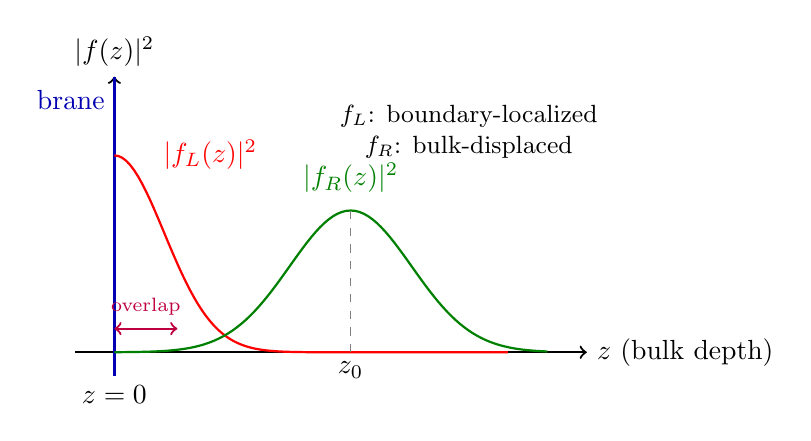
\begin{tikzpicture}[scale=1.0]
    % Axes
    \draw[->, thick] (-0.5,0) -- (6,0) node[right] {$z$ (bulk depth)};
    \draw[->, thick] (0,-0.3) -- (0,3.5) node[above] {$|f(z)|^2$};

    % Brane at z=0
    \draw[very thick, blue!70!black] (0,-0.3) -- (0,3.5);
    \node[blue!70!black, left] at (0,3.2) {brane};
    \node[below] at (0,-0.3) {$z=0$};

    % Left-handed profile (peaked at z=0)
    \draw[thick, red, domain=0:5, samples=100]
        plot (\x, {2.5*exp(-\x*\x/0.8)});
    \node[red, above right] at (0.5,2.2) {$|f_L(z)|^2$};

    % Right-handed profile (peaked at z=z_0)
    \draw[thick, green!50!black, domain=0:5.5, samples=100]
        plot (\x, {1.8*exp(-(\x-3)*(\x-3)/1.2)});
    \node[green!50!black, above] at (3,1.9) {$|f_R(z)|^2$};

    % z_0 marker
    \draw[dashed, gray] (3,0) -- (3,1.8);
    \node[below] at (3,0) {$z_0$};

    % Overlap region annotation
    \draw[<->, thick, purple] (0,0.3) -- (0.8,0.3);
    \node[purple, above, font=\scriptsize] at (0.4,0.35) {overlap};

    % Annotation
    \node[align=center, font=\small] at (4.5,2.8)
        {$f_L$: boundary-localized\\$f_R$: bulk-displaced};
\end{tikzpicture}
\caption{\textbf{Schematic of chiral mode profiles (not a fit).}
The left-handed mode $f_L(z)$ is peaked at the boundary $z=0$.
The right-handed mode $f_R(z)$ is displaced to $z = z_0$ deep in the bulk.
The overlap of $f_R$ with the boundary is exponentially suppressed.
This illustrates why only left-handed fermions couple to boundary-localized
gauge fields.}
\label{fig:ch9_overlap_schematic}
\end{figure}

% ==============================================================================
\subsection{Effective 4D Coupling and V–A Emergence}
\label{sec:ch9_va_emergence}

Now we return to the exact solutions and derive the V$-$A structure.

\subsubsection{Effective 4D Interaction}

\textbf{The principle:} If a weak mediator field $W_\mu$ couples to fermions at
the brane interface, the effective 4D coupling is proportional to the overlap integral.

\textbf{The overlap integrals:}
\begin{equation}
    g_{\text{eff}}^{(L)} \propto \int_0^L |f_L(z)|^2 \, dz
    \qquad
    g_{\text{eff}}^{(R)} \propto \int_0^L |f_R(z)|^2 \, dz
    \label{eq:ch9_overlap}
\end{equation}

\textbf{For left-handed modes:} Since $f_L$ is localized near $z=0$ and
normalizable, $g_{\text{eff}}^{(L)} = O(1)$. The full coupling survives.

\textbf{For right-handed modes:} Since $f_R$ grows into the bulk and is not
normalizable, $g_{\text{eff}}^{(R)} \to 0$ (or is exponentially suppressed if
we cut off the integral).

\subsubsection{The V–A Current Structure}

\textbf{The effective Lagrangian.} Putting left and right together, the
effective 4D weak interaction takes the form:
\begin{equation}
    \mathcal{L}_{\text{eff}} \propto g_{\text{eff}}^{(L)} \bar\psi_L \gamma^\mu \psi_L \, W_\mu
    + g_{\text{eff}}^{(R)} \bar\psi_R \gamma^\mu \psi_R \, W_\mu
    \label{eq:ch9_L_eff}
\end{equation}

\textbf{With} $g_{\text{eff}}^{(R)} \approx 0$\textbf{:}
\begin{equation}
    \mathcal{L}_{\text{eff}} \propto \bar\psi_L \gamma^\mu \psi_L \, W_\mu
    = \bar\psi \gamma^\mu P_L \psi \, W_\mu
    = \frac{1}{2} \bar\psi \gamma^\mu (1 - \gamma^5) \psi \, W_\mu
    \label{eq:ch9_va_derived}
\end{equation}

This is the V$-$A structure.

\begin{tcolorbox}[edcCanonical, title=\textbf{V–A Structure Emergence [Dc]}]
The characteristic $V{-}A$ weak current structure:
\begin{equation}
    J^\mu_{\text{weak}} = \bar\psi \gamma^\mu (1 - \gamma^5) \psi
\end{equation}
emerges from the 5D geometry without being imposed. The only left-right
asymmetry input is the \textbf{sign} of the Plenum inflow, which determines
the sign of the mass profile.

\textbf{No chirality smuggling:} The chirality selection is a \emph{consequence}
of the inflow direction, not an assumption about gauge quantum numbers.
\end{tcolorbox}

% ==============================================================================
\subsection{Boundary Condition Interpretation}
\label{sec:ch9_boundary}

There is an equivalent way to state the result: in terms of boundary conditions.

\subsubsection{The Boundary Projection}

The chiral localization can equivalently be viewed through boundary conditions.
At the observer boundary $z = 0$, the EDC ``frozen regime'' imposes constraints
on fermion fields.

\paragraph{EDC boundary condition (interpretation).}
The condition that only left-handed modes couple to observer physics is
equivalent to a boundary projection:
\begin{equation}
    P_R \psi\big|_{\text{boundary}} = 0
    \qquad \text{or} \qquad
    (1 + \gamma^5) \psi\big|_{z \to 0} \to 0
    \label{eq:ch9_bc}
\end{equation}

\textbf{Important:} This is \emph{not} imposed by hand; it emerges from the
normalizability requirement for modes in the domain-wall background.

\subsubsection{Comparison with MIT Bag}

\paragraph{Comparison with MIT bag.}
The MIT bag boundary condition for quark confinement has the form
$(1 - i\gamma^5 \hat{n} \cdot \gamma)\psi|_{\text{surface}} = 0$.
While structurally similar, the EDC mechanism is distinct: it arises from
mode localization in an asymmetric mass background, not from imposing
confinement on a bag surface. We note the analogy but do not claim equivalence \tagI{}.

% ==============================================================================
\subsection{Minimal SU(2)$_L$ Gauge Embedding}
\label{sec:ch9_su2_embedding}

\textbf{Why here?} After establishing the chirality filter and showing that overlap
determines coupling, we now fix \emph{where} SU(2)$_L$ lives and \emph{how} it couples.
This is not a new derivation direction---it completes the geometric picture by specifying
the gauge field location. We do \textbf{not} derive SM gauge symmetry origin here.

\medskip

In this chapter we derived the $V{-}A$ structure from 5D chiral localization:
left-handed modes remain boundary-supported while right-handed modes are displaced
into the bulk. What is still missing is a minimal statement of \emph{where} the
SU(2)$_L$ gauge fields live and \emph{how} they couple to these localized fermions.

We therefore adopt the simplest consistent embedding \tagP{}:
\begin{quote}
\textbf{Postulate:} The SU(2)$_L$ gauge fields $W_\mu^a$ are \emph{brane-localized}
at the observer boundary.
\end{quote}

\subsubsection{Coupling from Brane-Localized Action}

\textbf{The action.} The brane-localized gauge action takes the form:
\begin{equation}
    S \supset \int d^4x\,dz\,\delta(z)\,\Big(-\tfrac{1}{4} W^a_{\mu\nu}W^{a\mu\nu}
    + \bar{g}_2\,W^a_\mu J_L^{a\mu}\Big)
    \label{eq:ch9_brane_gauge_action}
\end{equation}
where $J_L^{a\mu} = \bar\Psi_L \gamma^\mu T^a \Psi_L$ is the left-handed current.

\textbf{The integration.} Integrating over $z$ with normalized fermion profiles
$f_L(z)$ gives the effective coupling:
\begin{equation}
    g_{\text{eff}} \propto \bar{g}_2 \int dz\,|f_L(z)|^2\,\delta(z)
    \quad\Rightarrow\quad
    g_{\text{eff}} \simeq g_2 \quad \text{(up to brane kinetic terms)}
    \label{eq:ch9_geff}
\end{equation}

\textbf{The result:}
\begin{itemize}[nosep]
    \item For \textbf{left-handed modes} (boundary-supported), the overlap is
          $\mathcal{O}(1)$, giving full gauge coupling.
    \item For \textbf{right-handed modes} (bulk-displaced), the overlap is
          exponentially suppressed by their displacement from the boundary.
\end{itemize}

This immediately aligns the gauge interaction with the chirality filter derived
earlier: SU(2)$_L$ couples strongly to left-handed doublets and negligibly to
right-handed singlets.

\subsubsection{Alternative: Bulk Gauge Fields}

An alternative embedding would have gauge fields propagate in the full 5D bulk,
coupling to fermions everywhere. This would require:
\begin{itemize}[nosep]
    \item Kaluza--Klein reduction of 5D gauge fields
    \item A separate localization mechanism for gauge zero modes
    \item Additional assumptions about bulk gauge dynamics
\end{itemize}
We do not pursue this here; the brane-localized ansatz is \emph{minimal} \tagP{}.
If future work requires bulk gauge propagation (e.g., for gauge unification or
KK tower signatures), the brane-localized limit is recoverable as the leading-order term.

\subsubsection{No-Smuggling Guardrail}

\begin{tcolorbox}[colback=red!5!white, colframe=red!50!black, title=Epistemic Status: SU(2)$_L$ Embedding]
\small
\begin{tabular}{lll}
\toprule
\textbf{Item} & \textbf{Status} & \textbf{Note} \\
\midrule
SU(2)$_L$ brane-localization & \tagP{} & Postulated, not derived \\
Overlap coupling $g_{\text{eff}} \simeq g_2$ & \tagP{} & From brane action ansatz \\
Consistency with V--A & \tagDc{} & Follows from Ch.9 chirality mechanism \\
Origin of gauge symmetry & (open) & Why SU(2)$_L$? Not addressed \\
W$^\pm$/Z$^0$ mass generation & (open) & Higgs mechanism not derived \\
Gauge coupling $g_2$ value & \tagBL{} & Input from SM \\
\bottomrule
\end{tabular}
\end{tcolorbox}

\subsubsection{Verdict}

\begin{tcolorbox}[colback=yellow!5!white, colframe=yellow!60!black,
    title=OPR-17: Minimal SU(2)$_L$ Embedding]
\textbf{Status: YELLOW [P]} --- where/how fixed; origin + masses remain OPEN.

\begin{itemize}[nosep]
    \item \textcolor{OliveGreen}{\textbf{GREEN:}} Consistent with existing V--A chirality filter \tagDc{}
    \item \textcolor{YellowOrange}{\textbf{YELLOW:}} Brane-localized SU(2)$_L$ + overlap coupling \tagP{}
    \item \textcolor{BrickRed}{\textbf{RED/OPEN:}} Gauge symmetry origin; W$^\pm$/Z$^0$ mass generation
\end{itemize}

\medskip
\noindent\fbox{\parbox{0.94\textwidth}{\small
\textbf{SU(2)$_L$ embedding (OPR-17):} Brane-localized gauge fields couple to
boundary-supported left-handed modes with $g_{\text{eff}} \simeq g_2$; right-handed
modes decouple by bulk displacement. This fixes ``where/how'' without deriving
gauge symmetry origin or mass generation.}}
\end{tcolorbox}

% ==============================================================================
\subsection{Dimensional and Consistency Checks}
\label{sec:ch9_consistency}

\begin{tcolorbox}[colback=gray!5!white, colframe=gray!60!black,
    title=\textbf{Consistency Check (Not a Derivation)}]
This section verifies internal consistency. It contains no new physics claims.
\end{tcolorbox}

\paragraph{Dimension check.}
\begin{itemize}[nosep]
    \item $[\Psi] = [\text{mass}]^2$ in 5D (for canonically normalized action)
    \item $[f_{L/R}(z)] = [\text{mass}]^{1/2}$ (profile function)
    \item $[\psi_{L/R}(x)] = [\text{mass}]^{3/2}$ in 4D (standard 4D spinor)
    \item $[m(z)] = [\text{mass}]$ (5D mass profile)
    \item $[\lambda] = [\text{length}]$ (localization scale)
\end{itemize}
The mode expansion~\eqref{eq:ch9_mode_expansion} and solutions~\eqref{eq:ch9_fL_sol}--\eqref{eq:ch9_fR_sol} are dimensionally consistent.

\paragraph{Convention independence.}
The V–A result depends only on:
\begin{enumerate}[nosep]
    \item The \emph{sign} of $m(z)$ for $z > 0$, determined by inflow direction
    \item The standard definition of $\gamma^5$ and chiral projectors
\end{enumerate}
There is no dependence on factors of $4\pi$ or electromagnetic coupling $\alpha$.

% ==============================================================================
\subsection{Summary}
\label{sec:ch9_summary}

% --- THREE TAKEAWAYS (Feynman style) ---

\begin{tcolorbox}[colback=blue!5!white, colframe=blue!50!black,
    title=\textbf{Three Takeaways}]
\begin{enumerate}
    \item \textbf{Chirality is geometry.}
          The weak interaction's left-handedness is not an arbitrary choice---it follows
          from how fermion modes localize in the extra dimension. Plenum inflow picks
          a sign; that sign determines which chirality sits at the boundary.

    \item \textbf{V–A emerges from overlap.}
          Gauge fields on the brane couple only to what overlaps with them. Left-handed
          modes peak at the brane; right-handed modes are pushed into the bulk. The
          result is automatic V–A without imposing it by hand.

    \item \textbf{No new parameters.}
          This mechanism uses standard 5D Dirac physics \tagBL{} plus one EDC postulate
          (inflow direction) \tagP{}. No chirality-specific coupling constants are introduced.
\end{enumerate}
\end{tcolorbox}

\medskip

% --- WHAT REMAINS OPEN ---

\begin{tcolorbox}[colback=red!5!white, colframe=red!50!black,
    title=\textbf{What Remains Open}]
\begin{itemize}[nosep]
    \item \textbf{Gauge symmetry origin:} Why SU(2)$_L$ specifically? (OPR-17, partial)
    \item \textbf{W$^\pm$/Z$^0$ masses:} Higgs mechanism not derived from EDC.
    \item \textbf{Fermi constant:} Quantitative $G_F$ requires thick-brane profile (Ch.~11).
    \item \textbf{Mixing matrices:} CKM/PMNS from generational overlaps (OPR-18).
    \item \textbf{Neutrino mass:} Majorana vs.\ Dirac structure (OPR-07).
\end{itemize}
\end{tcolorbox}

\medskip

% --- DETAILED AUDIT TABLE ---

\begin{tcolorbox}[colback=green!5, colframe=green!50!black,
    title=\textbf{Epistemic Audit}]
\begin{center}
\small
\begin{tabular}{lll}
\toprule
\textbf{Element} & \textbf{Source} & \textbf{Status} \\
\midrule
5D Dirac equation & Standard QFT & \tagBL{} \\
Chiral projectors $P_{L/R}$ & Standard QFT & \tagBL{} \\
Domain wall localization & Jackiw--Rebbi/Kaplan & \tagBL{} \\
Plenum inflow direction & EDC Framework v2.0 & \tagP{} \\
Fermion-stress coupling $m(z) \sim \kappa T^{zz}$ & Physical hypothesis & \tagP{} \\
$m(z) > 0$ for $z > 0$ & From inflow direction & \tagDc{} \\
$f_L$ localized at boundary & Mathematical consequence & \tagDc{} \\
$f_R$ expelled into bulk & Mathematical consequence & \tagDc{} \\
V–A current structure & Emerges from above & \tagDc{} \\
MIT bag analogy & Structural comparison & \tagI{} \\
\bottomrule
\end{tabular}
\end{center}
\end{tcolorbox}

